\clearpage
\section{Opis realizacji}
\label{sec:opis_realizacji}

\quad Realizacja zadań projektowych opisanych w rozdziale \ref{sec:koncepcja} została przeprowadzona przy użyciu wszystkich technologii, które są wymienione w rozdziale \ref{sec:spec_prog}. Można ją podzielić na trzy główne części, które zostaną przedstawione w kolejnych podrozdziałach.

\subsection{Konfiguracja wirtualnego środowiska}
\label{sub:konfiguracja}
\quad Pierwszym elementem, który należało opanować było uruchomienie wirtualnej maszyny ,,TangoBox9'', a następnie konfiguracja wszystkich elementów niezbędnych do realizacji postawionego celu. Kolejne kroki postępowania zostały przedstawione poniżej:

\begin{enumerate}
	\item Sprawdzenie funkcjonowania systemu Tango: głównej bazy danych, poszczególnych ,,serwerów urządzeń'' (ang. device servers) oraz samych urządzeń. W tym celu użyto dwóch aplikacji stanowiących pakiet do zarządzania systemem Tango: Astor i Jive. Weryfikacja poprawności polegała na uruchomieniu obu aplikacji i wizualnym sprawdzeniu stanów interesujących z punktu widzenia projektu komponentów systemu.
	\item Sprawdzenie funkcjonowania dodatków do systemu Tango: archiwizacji, bibliotek Taurus i Sardana. Należało uruchomić odpowiednie aplikacje (,,jhdbconfigurator'' w przypadku archiwizacji, ,,taurusgui'' - Taurusa i ,,Sardemo'' - Sardany) i sprawdzić, czy nie wyrzucają jakiś błędów.
	\item Uruchomienie serwerów urządzeń zarządzających silnikami. Klasa ,,Motors'' jest częścią oprogramowania ,,Pool'', które należy do pakietu Sardana. Program Astor umożliwia włączenie serwera.
	\item Konfiguracja silników. Jej część jest automatycznie wprowadzana w czasie uruchomienia serwera urządzeń, jednak pewne parametry trzeba ustawić samemu. Zostały ustawione następujące elementy:
	\begin{enumerate}
		\item urządzenie ,,motor/motctrl01/1'':
		\begin{enumerate}
			\item zakres wartości położenia: -120, 120,
			\item progi alarmowe: -110, 110,
			\item progi ostrzeżeń: -100, 100,
			\item pozycje czujników krańcowych - takie, jak zakresy wartości położenia,
			\item prędkość: 10,
			\item przyspieszenie: 0,5.
		\end{enumerate}
		\item urządzenie ,,motor/motctrl01/2'':
		\begin{enumerate}
			\item zakres wartości położenia: -120, 120,
			\item progi alarmowe: -110, 110,
			\item progi ostrzeżeń: -100, 100,
			\item pozycje czujników krańcowych - takie, jak zakresy wartości położenia,
			\item prędkość: 100,
			\item przyspieszenie: 40.
		\end{enumerate}
		\item urządzenie ,,motor/motctrl01/3'':
		\begin{enumerate}
			\item zakres wartości położenia: -50, 50,
			\item progi alarmowe: -45, 45,
			\item progi ostrzeżeń: -40, 40,
			\item pozycje czujników krańcowych - takie, jak zakresy wartości położenia,
			\item prędkość: 10,
			\item przyspieszenie: 0,1.
		\end{enumerate}
		\item urządzenie ,,motor/motctrl01/4'':
		\begin{enumerate}
			\item zakres wartości położenia: -90, 140,
			\item progi alarmowe: -85, 130,
			\item progi ostrzeżeń: -80, 125,
			\item pozycje czujników krańcowych - takie, jak zakresy wartości położenia,
			\item prędkość: 100,
			\item przyspieszenie: 1.
		\end{enumerate}
	\end{enumerate}
	
	\item Dodanie odpowiednich parametrów do archiwizacji. Wirtualna maszyna ,,TangoBox9'' zawiera system archiwizacji ,,HDB++'', który został przygotowany przez zespół synchrotronu Elettra we Włoszech. Dostarczone są do niego dwie aplikacje: ,,jhdbconfigurator'' (służąca do wprowadzania zmian w konfiguracji archiwizacji) oraz ,,jhdbviewer'' (wykorzystywana do podglądu archiwizowanych atrybutów). Za pomocą pierwszej z nich ustawiono archiwizację położeń i pozycji czujników krańcowych każdego silnika. Druga aplikacja została zaprezentowana na rysunku \ref{fig:Archiving}.
	
	\item Następnie dokonano sprawdzenia działania urządzeń nadrzędnych nad zwykłymi silnikami - tzw. ,,pseudo-silników'' (ang. PseudoMotors). System Tango wspiera hierarchiczność urządzeń, a więc synchronizację pracy poszczególnych silników najprościej jest zrealizować właśnie w takiej formie. Użyto domyślnych ustawień, obecnych w symulacji środowiska linii pomiarowej, jakie jest dostarczone z pakietem Sardana.
	
	Skonfigurowano dwa pseudo-silniki: ,,slit'' i ,,gap''. Oba synchronizują pracę pierwszych dwóch silników. Pierwszy może być interpretowany jako ustawienie wielkości szczeliny, przez którą pada światło, a drugi służy do realizowania przesunięcia między dwoma symetrycznymi elementami, którymi te silniki poruszają.
\end{enumerate}

\begin{figure}[ht]
	\begin{adjustbox}{addcode={
				\begin{minipage}{\width}}
				{\caption{Zrzut ekranu przedstawiający aplikację wyświetlającą dane archiwalne położenia silników.}\label{fig:Archiving}
				\end{minipage}},rotate=90,center}
			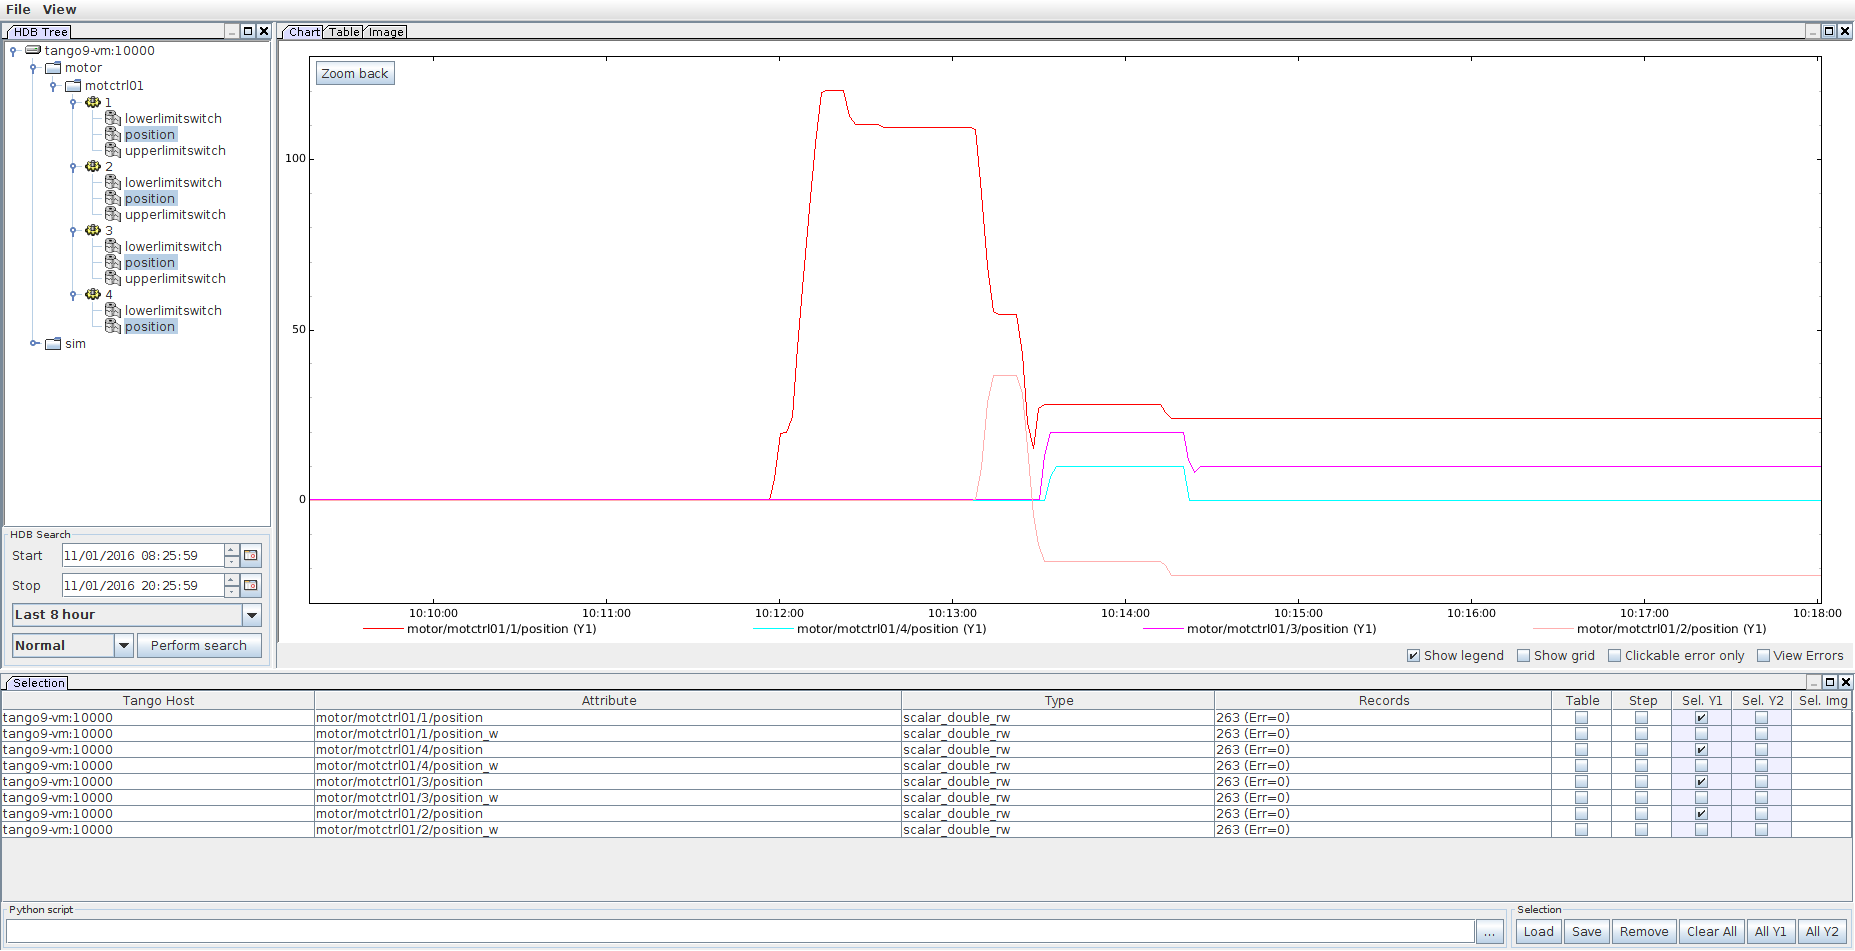
\includegraphics[scale=.32]{Grafika/ArchivingMotors}
	\end{adjustbox}
\end{figure}

\subsection{Opracowanie aplikacji eksperckiej i operatorskiej}
\label{sub:apps}

\quad Druga część realizacji zagadnień projektowych obejmowała utworzenie obu wymaganych aplikacji realizujących dwa odrębne sposoby wizualizacji wartości położeń wałów silników. Dodatkowo, w pracy nad nimi wykorzystano dwa możliwe sposoby tworzenia aplikacji w pakiecie TaurusGUI.

Pierwszy sposób to podejście konfiguracyjne. Użytkownik nie musi pisać kodu aplikacji - jest on generowany niejawnie za niego. Tak powstała aplikacja ekspercka: uruchomiono kreator GUI poleceniem: ,,\texttt{taurusgui --new}'' i ustawiono konkretne panele, które miały się w niej znajdować. Następnie ustawiono odpowiednią perspektywę (o nazwie ,,ExpertGUI'') i dodatkowe panele, które użytkownik może sam dołączyć do aplikacji w czasie jej działania.

Kolejnym krokiem była konfiguracja panelu z wykresem oraz zapisanie ustawień, które zawierały między innymi: odpowiednie sygnały, ich nazwy, kolory na wykresie i skalę. Ostatnią czynnością było utworzenie i zapisanie przykładowej sekwencji makr. Oba wspomniane wyżej pliki konfiguracyjne zostały dołączone do plików projektowych i są opisane w rozdziale \ref{sec:opis_kodu}.

Drugi możliwy sposób tworzenia interfejsów użytkownika przy pomocy pakietu Taurus to podejście programistyczne. Najpierw stworzono szkielet wyglądu aplikacji przy pomocy programu QtDesigner. Wygenerowany plik z rozszerzeniem .ui (z ang. user interface - interfejs użytkownika) można albo bezpośrednio zaimportować do aplikacji w Pythonie, albo skonwertować na kod w tym języku. Wybrany został drugi sposób postępowania, jako że importowany plik .ui nie zawierał wszystkich potrzebnych elementów. Przede wszystkim, stworzenia wymagał drugi sposób wizualizacji, czyli klasa realizująca wyświetlanie w czasie rzeczywistym wartości położenia silników. Pisanie kodu i testowanie prototypów aplikacji w znaczącym stopniu ułatwiło korzystanie z zaawansowanego środowiska programistycznego, jakim jest PyCharm.

Dokładny opis obu aplikacji znajduje się w rozdziale \ref{sec:manual}.


\subsection{Testy}